\documentclass[a4paper]{scrartcl}
\usepackage[cm]{fullpage}
\usepackage{amsmath, amssymb, esint}
\usepackage{siunitx}

\usepackage{tikz, pgfplots, pgfplotstable}
\pgfplotsset{
    compat = 1.12,
    plot-scatter/.style = {
        only marks,
        error bars/.cd,
        x dir = both, y dir = both,
        x explicit, y explicit
    }
}

\pgfplotstableread{part1.tsv}\partonetsv

\begin{document}

\title{PHYS3112: Acousto-optics}
\author{ \\ \\ }
\date{2017-05-15}
\maketitle

\begin{abstract}
    We observe Bragg deflection and intensity modulation of a \SI{633}{\nano\metre} laser signal using acousto-optics. Bragg's law seems to hold, and we get a very good SNR for modulation in the audible range.
\end{abstract}

\section{Materials and Methods}
Please refer to the student notes of the experiment.

The laser used was a standard HeNe \(\lambda = \SI{633}{\nano\metre}\) laser.

\subsection{Part 1: Bragg Deflection}
The screen was placed \(L = \SI{140 \pm 1}{\centi\metre}\) away from the deflector.

The Bragg deflection angle is given by:
\[\frac{\lambda}{v} f = \sin \theta = \sin \tan^{-1} \frac{d}{L}\]
where \(v\) is the speed of sound in the deflector, \(f\) the applied frequency, and \(d\) the 1st-to-0th order distance.

Since our values for \(d\) are two orders of magnitude smaller than \(L\), we can use the small angle approximation to get:
\[\frac{\lambda L}{v} f \approx d\]

To find the speed of sound \(v\), we can take the linear regression between \(d\) and \(f\), and then solve for \(v\) in the gradient \(\frac{\lambda L}{v}\).

The manual for the deflector indicates the deflector will deflect at an angle of \(\theta = \SI{11.4}{\milli\radian}\) at \(f = \SI{70}{\mega\hertz}\) and \(\lambda = \SI{633}{\nano\metre}\). This corresponds to a speed of sound of \(v = \SI{3890}{\metre\per\second}\).

\subsection{Part 2: Modulation}
The photodiode was placed \(L = \SI{180 \pm 1}{\centi\metre}\) away from the modulator.

The input signal was maintained as a sine wave with frequency \(f = \SI{400}{\hertz}\) and peak-to-peak voltage of \(V_{pp} = \SI{100}{\milli\volt}\) for all measurements.

Note that the notes use an incorrect definition for signal-to-noise ratio. What they mean by signal-to-noise ratio is actually a AC peak-to-peak to DC offset ratio. Both values have been calculated, to show the stark difference between them.

\section{Results}
\subsection{Part 1: Bragg Deflection}
\begin{figure}
    \centering
    \begin{tikzpicture}
        \begin{axis}[
            xlabel = \(f\) (\si{\mega\hertz}),
            ylabel = \(d\) (\si{\milli\metre})
        ]
            \addplot +[plot-scatter] table [
                x expr = \thisrowno{0},
                x error expr = 0,
                y expr = \thisrowno{1},
                y error expr = \thisrowno{2}
            ] {\partonetsv};
            \addplot +[no marks, domain = 40:110] {0.237499 * x};
            \addplot [no marks, domain = 40:110] {0.243166 * x};
            \addplot [no marks, domain = 40:110] {0.231832 * x};
            \addplot [green, no marks, domain = 40:110] {0.227815 * x};
        \end{axis}
    \end{tikzpicture}
    \caption{1st-to-0th order distance \(d\) by frequency applied to the deflector \(f\). Red/black: Fitted line; Green: Expected line}
    \label{fig:part1}
\end{figure}

The measured deflection distances (1st-to-0th order) can be seen in Figure \ref{fig:part1}.

Performing a linear regression results in a gradient of \SI{0.237 \pm 0.006}{\milli\metre\per\mega\hertz}, corresponding to a speed of sound of \(v = \SI{3730 \pm 90}{\metre\per\second}\). This is approximately \SI{96}{\percent} of the expected value.

\subsection{Part 2: Modulation}
\begin{table}
    \centering
    \begin{tabular}{c | c | c | c | c | c}
        Order & Background \(I_{DC}\) (\si{\milli\ampere}) & Un/modulated \(I_{DC}\) (\si{\milli\ampere}) & \(I_{PP}\) (\si{\milli\ampere}) & \(\frac{I_{PP}}{I_{DC}}\) (\si{\decibel}) & SNR (\si{\decibel}) \\
        \hline
        0 & \SI{44 \pm 2}{} & \SI{471 \pm 1}{} & \SI{1.9 \pm 0.1}{} & \SI{-23.9 \pm 0.2}{} & \SI{11 \pm 1}{} \\
        1 Left & \SI{56 \pm 1}{} & \SI{66 \pm 1}{} & \SI{8.3 \pm 0.1}{} & \SI{-9.00 \pm 0.08}{} & \SI{40 \pm 1}{} \\
        1 Right & \SI{63 \pm 1}{} & \SI{316 \pm 1}{} & \SI{25.6}{} & \SI{-10.914 \pm 0.014}{} & \SI{48 \pm 1}{}
    \end{tabular}
    \caption{Current and SNR measurements of the photodiodes}
    \label{tab:part2}
\end{table}

\begin{figure}
    \centering
    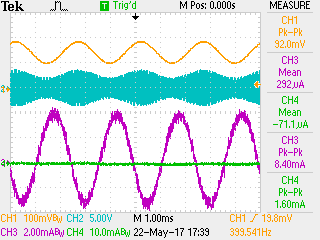
\includegraphics[width = 8cm]{1st-left-amp.png}
    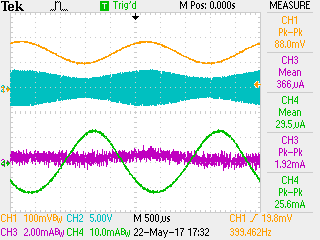
\includegraphics[width = 8cm]{1st-right-amp.png}
    \caption{The amplitude readings. CH1: Input signal; CH2: Modulated signal; Left CH4 and Right CH3: 0th order photodiode; Left CH3: 1st left order photodiode; Right CH4: 1st right order photodiode}
    \label{fig:part2-1st-amp}
\end{figure}

\begin{figure}
    \centering
    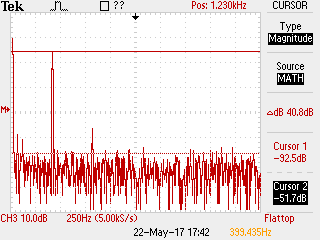
\includegraphics[width = 8cm]{1st-left-fft.png}
    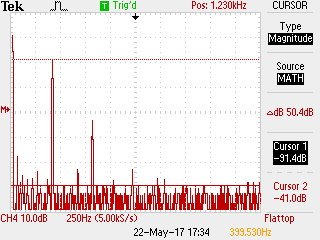
\includegraphics[width = 8cm]{1st-right-fft.png}
    \caption{The frequency spectrum of the 1st left and right spots, respectively. The three peaks are the DC offset, the \SI{400}{\hertz} fundamental, and the \SI{800}{\hertz} 1st harmonic.}
    \label{fig:part2-1st-fft}
\end{figure}

The 1st-to-0th order distance was \SI{31.8 \pm 1.0}{\milli\metre}, and the photodiode placed at these points. This distance corresponds to a speed of sound in the modulator of \SI{3070 \pm 100}{\metre\per\second}. This is about \SI{85}{\percent} of the value of \SI{3630}{\metre\per\second} quoted in the manual.

The angle of the modulator was adjusted such that the 1st right order maxima was as bright as possible.

If the input signal DC offset was adjusted, there was perfect frequency doubling occurring around a DC offset of \SI{0}{\volt}. Other than that in the full available range of -1.9 to \SI{1.9}{\volt}, no other distortion was observed.

The DC offset was set to \SI{159 \pm 1}{\milli\volt} (this produced the best SNR) and the measurements shown in Table \ref{tab:part2}. The only harmonic distortion observed was a first harmonic, which had a amplitude of \SI{-28.4}{\decibel} of the fundamental. Many of the observations were taken from oscilloscope graphs looking like Figures \ref{fig:part2-1st-amp} and \ref{fig:part2-1st-fft}.

\section{Discussion}
\subsection{Part 1: Bragg Deflection}
The deflection distance verses signal frequency graph is very linear and produced a very good fit, as expected.

Our speed of sound result of \(v = \SI{3730 \pm 90}{\metre\per\second}\) was \SI{96}{\percent} of the expected value of \SI{3890}{\metre\per\second}, which was most likely caused by a poor measurement of the deflector-to-screen length \(L\). It was difficult to measure this length accurately, since our measuring tape incurred a significant bend (due to gravity), artificially increasing the measured length, causing a smaller-than-expected speed of sound value.

But otherwise, it is quite a good result, indicating accuracy of Bragg's law.

\subsection{Part 2: Modulation}
Once again, our speed of sound is a little bit too small, at \SI{85}{\percent} of the value of \SI{3630}{\metre\per\second} quoted in the manual. This probably is the result of a combination of overestimating the modulator-to-diode length and underestimating the diode-to-diode (1st-to-0th order) separation.

At a DC offset around \SI{0}{\volt}, the frequency doubling observed is completely expected, as the input signal is now oscillating between both positive and negative voltages. The modulator simply multiplies the signal with the modulation frequency, while the demodulator takes the absolute envelope. This means the modulator-demodulator pair basically acts as a absolute value function on the input signal (ignoring possible distortion), and taking the absolute value of a sinusoidal centered around 0 can be trivially seen to double its frequency.

No other kinds of distortion was observed most likely due to measuring completely within the operating specifications of the modulator and demodulator, where the manufacturer would have guaranteed them to be linear in that region. If we measured outside of the operating specifications, maybe other distortions (such as clipping) might be observed.

Both the unmodulated and modulated currents as measured by the diodes (Table \ref{tab:part2}) have equal currents, as expected, since modulation does not change the average intensity (DC offset) of the output. One would expect the peak-to-peak current of the 0th order diode to equal to the sum of the two 1st orders, since the light either goes to the 0th order or the 1st, but this is not the case since the diode is not linear. It seems the diode is much more sensitive to intensity changes at low intensity. Correspondingly, we have a better SNR for the signals with intensity, though only to a certain point where background noise starts drowning out the signal.

The best SNR of \SI{48 \pm 1}{\decibel} would likely be hitting the 16-bit ADC limitation of the oscilloscope (where the ``noise'' measured would simply be quantisation noise), indicating an outstanding SNR.

\section{Conclusion}
\emph{(From abstract)} We observe Bragg deflection and intensity modulation of a \SI{633}{\nano\metre} laser signal using acousto-optics. Bragg's law seems to hold, and we get a very good SNR for modulation in the audible range.

\end{document}